\section{Analysis}
\label{sec:analysis}

%TODO(pm):Make new table
\setlength{\tabcolsep}{3pt}
\begin{table}
\scriptsize
\begin{tabular}{l|r|r|r|r|r}

Game &          SimPLe (ours)  &     rainbow\_100k &     ppo\_500k   &     human &          random \\

\midrule
Alien          &    405.2 &    290.6 &    269.0 &   7128.0 &   184.8 \\
Amidar         &     88.0 &     20.8 &     93.2 &   1720.0 &    11.8 \\
Assault        &    369.3 &    300.3 &    552.3 &    742.0 &   233.7 \\
Asterix        &   1089.5 &    285.7 &   1085.0 &   8503.0 &   248.8 \\
BankHeist      &      8.2 &     34.5 &    641.0 &    753.0 &    15.0 \\
BattleZone     &   5184.4 &   3363.5 &  14400.0 &  37188.0 &  2895.0 \\
Boxing         &      9.1 &      0.9 &      3.5 &     12.0 &     0.3 \\
Breakout       &     12.7 &      3.3 &     66.1 &     30.0 &     0.9 \\
ChopperCommand &   1246.9 &    776.6 &    860.0 &   7388.0 &   671.0 \\
CrazyClimber   &  39827.8 &  12558.3 &  33420.0 &  35829.0 &  7339.5 \\
DemonAttack    &    169.5 &    431.6 &    216.5 &   1971.0 &   140.0 \\
Freeway        &     20.3 &      0.1 &     14.0 &     30.0 &     0.0 \\
Frostbite      &    254.7 &    140.1 &    214.0 &      - &    74.0 \\
Gopher         &    771.0 &    748.3 &    560.0 &   2412.0 &   245.9 \\
Hero           &   1295.1 &   2676.3 &   1824.0 &  30826.0 &   224.6 \\
Jamesbond      &    125.3 &     61.7 &    255.0 &    303.0 &    29.2 \\
Kangaroo       &    323.1 &     38.7 &    340.0 &   3035.0 &    42.0 \\
Krull          &   4539.9 &   2978.8 &   3056.1 &   2666.0 &  1543.3 \\
KungFuMaster   &  17257.2 &   1019.4 &  17370.0 &  22736.0 &   616.5 \\
MsPacman       &    762.8 &    364.3 &    306.0 &   6952.0 &   235.2 \\
Pong           &      5.2 &    -19.5 &     -8.6 &     15.0 &   -20.4 \\
PrivateEye     &     58.3 &     42.1 &     20.0 &  69571.0 &    26.6 \\
Qbert          &    559.8 &    235.6 &    757.5 &  13455.0 &   166.1 \\
RoadRunner     &   5169.4 &    524.1 &   5750.0 &   7845.0 &     0.0 \\
Seaquest       &    370.9 &    206.3 &    692.0 &  42055.0 &    61.1 \\
UpNDown        &   2152.6 &   1346.3 &  12126.0 &  11693.0 &   488.4 \\

\end{tabular}
\caption{Mean scores obtained by our method (SimPLe) in comparison with Rainbow trained on 100K steps (400K frames) and PPO trained on 500K steps (2 millions frames). Details and extended numerical results are included in Appendix~\ref{numerical_results}.}
\label{tab:shortNumericalResults}
\end{table}

In this section, we analyze the results of our experiments. Our goals are to study how much model-based reinforcement learning can improve over the efficiency of current model-free deep reinforcement learning algorithms, analyze the quality of the predictions made by our model, and examine the design decisions in our method. Unless stated otherwise, we assume that SimPLe uses rollouts of length $50$ generated with the stochastic discrete model and is trained with $\gamma=0.95$ (see Section \ref{sec:training} and Section \ref{sec:policy_training}). 
%TODO(pm): Review last sentence

\subsection{Sample Efficiency}
The primary evaluation in our experiments studies the sample efficiency of SimPLe, in comparison with state-of-the-art model-free deep RL methods in the literature. To that end, we compare with  Rainbow~\cite{rainbow,DBLP:journals/corr/abs-1812-06110}, which represents the state-of-the-art Q-learning method for Atari games, and PPO~\cite{ppo}, a model-free policy gradient algorithm. The results of the comparison are presented in Figures \ref{fig:compare_dopamine} and \ref{fig:compare_ppo}. For each game, we plot the number of time steps needed for either Rainbow or PPO to reach the same score that our method reaches after $100$K interaction steps. The red line indicates $100$K steps: any bar larger than this indicates a game where the model-free method required more steps. SimPLe outperforms the model-free algorithms in terms of learning speed on nearly all of the games, and in the case of a few games, does so by over an order of magnitude. For some games, it reaches the same performance that our PPO implementation reaches at $10$M steps. This indicates that model-based reinforcement learning provides an effective approach to learning Atari games, at a fraction of the sample complexity.

\begin{figure}[t]
\centering
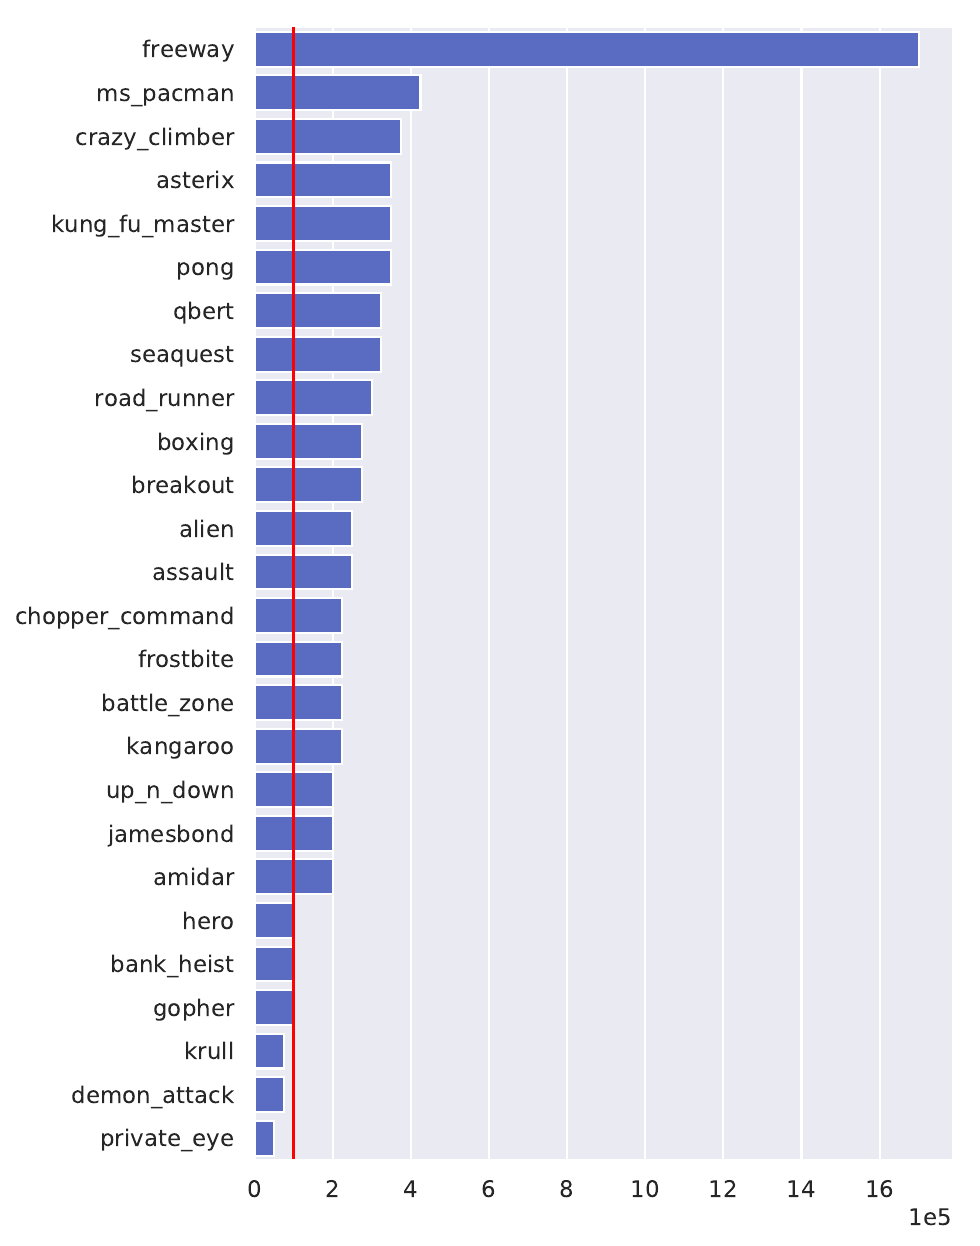
\includegraphics[width=1.0\columnwidth]{figures/v1_eval_longmodel_vs_rainbow-1.png}
\vspace{-0.2cm}
\caption{Comparison with Rainbow. Each bar illustrates the number of interactions with environment required by Rainbow to achieve the same score as our method (SimPLe). The red line indicates the $100$K interactions threshold which is used by the our method.} 
\label{fig:compare_dopamine}
\end{figure}

%TODO(pm): reveiew once tab:shortNumericalResults is done again
The results in these figures and Table \ref{tab:shortNumericalResults} are generated by averaging $5$ runs for each game. As shown in Table \ref{tab:shortNumericalResults}, the model-based agent is better than a random policy for all the games except \bankh. Interestingly, we observed that the best of the $5$ runs was often significantly better. For $6$ of the games, it exceed the average human score (as reported in Table 3 of \cite{Pohlenetal2018}). This suggests that further stabilizing model-based RL should improve performance, indicating an important direction for future work. In some cases during training  we observed high variance of the results during each step of the loop. There are a number of possible reasons, such as mutual interactions of the policy training and the supervised training or domain mismatch between the model and the real environment. We present detailed numerical results, including best scores and standard deviations, in Appendix \ref{numerical_results}.

\begin{figure}[t]
\centering
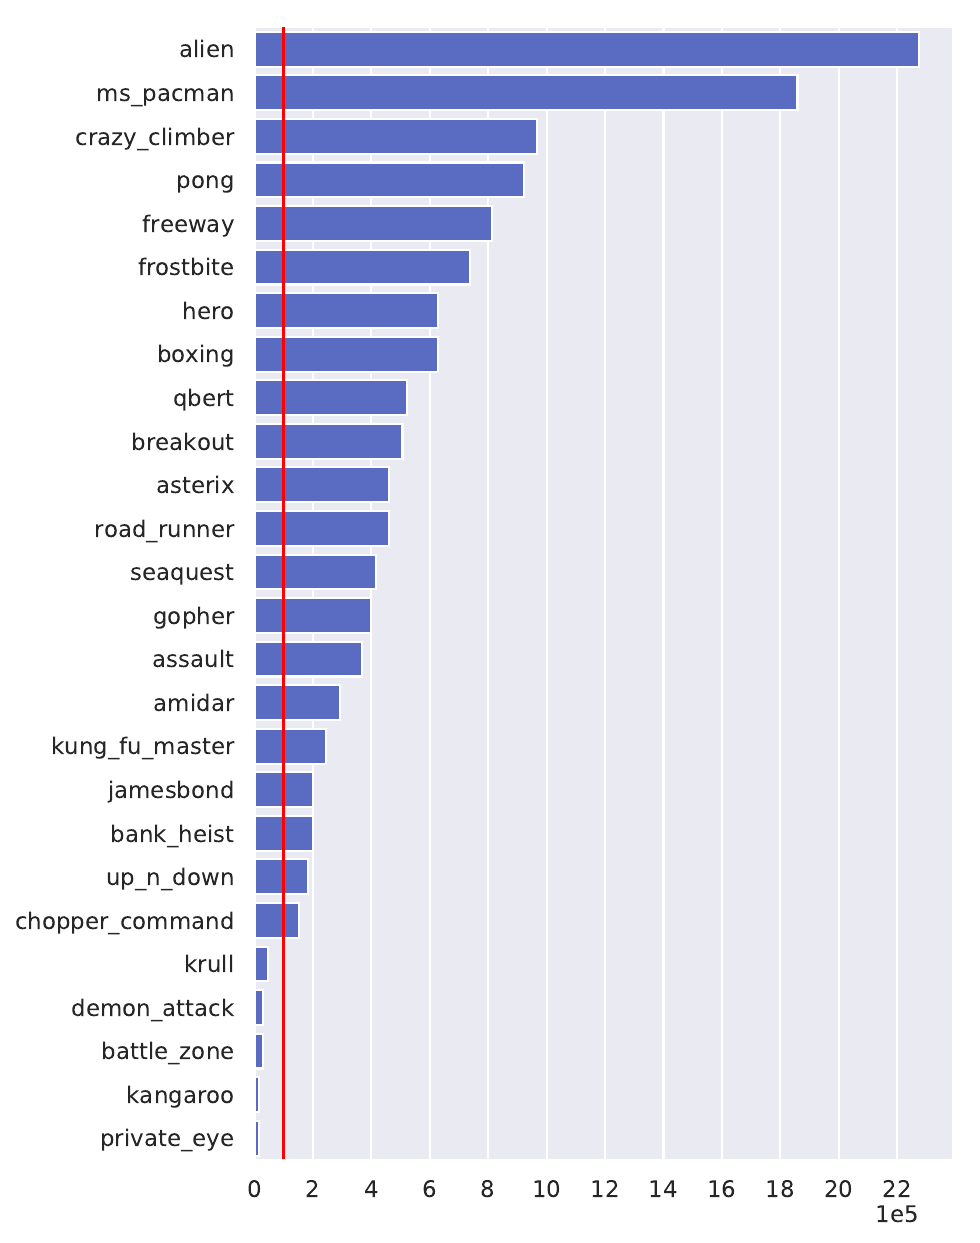
\includegraphics[width=1.0\columnwidth]{figures/v1_eval_longmodel_vs_ppo-1.png}
\caption{Comparison with PPO. Each bar illustrates the number of interactions with environment required by PPO to achieve the same score as our method (SimPLe). The red line indicates the $100$K interactions threshold which is used by the our method.}
\label{fig:compare_ppo}
\end{figure}

%TODO(pm): add the appendix
\textbf{Number of frames.} We focused our work on learning games with $100$K interaction steps with the environment, but we also studied settings with $20$K, $50$K, $200$K, $500$K and $1$M interactions. Our results are poor with $20$K interactions, but already almost as good with $50$K as with $100$K interactions. From there they improve with more interactions but above $200$K it becomes competitive to model-free RL starting from a policy pre-trained with SimPLe, see Appendix~\ref{appdx:num_samples} for details.

\subsection{Ablations}\label{sec:ablations}

To evaluate the design of our method, we independently varied a number of the design decisions: the choice of the model, the $\gamma$ parameter, the length of PPO rollouts and the length of model training.

As for choosing the \emph{model architecture}, we evaluated a few choices and our proposed stochastic discrete model performs best by a significant margin.
As for the number $N$ of \emph{steps} so that every $N$ steps we reinitialize the simulated environment with ground-truth data, we use $N=50$ by default. We experimented with $N=25$ or $N=100$ and $100$ is a bit worse than either $25$ or $50$ (which are on par), likely due to compounding model errors, but this effect is much smaller than the effect of model architecture. The \emph{discount factor} $\gamma=0.99$ unless specified otherwise.  We see that $\gamma=0.95$ is slightly better than other values, and we hypothesize that it is due to better tolerance to model imperfections. But overall, all three values of $\gamma$ perform comparably at the same number of steps.

\paragraph{Models.} To evaluate the model choice, we evaluated the following models: deterministic, deterministic recurrent, and stochastic discrete (see Section \ref{sec:architectures}). As can be seen, our proposed stochastic discrete model performs best. Figures \ref{fig:effects_stocha} and \ref{fig:comp_recurr} show the role of stochasticity and recurrence. 

\paragraph{Steps.} See Figures \ref{fig:adj_steps}. As described in Section \ref{sec:policy_training} every $N$ steps we reinitialize the simulated environment with ground-truth data. By default we use $N=50$, in some experiments 
we set $N=25$ or $N=100$. It is clear from the table above and Figure~\ref{fig:100steps} that $100$ is a bit worse than either $25$ or $50$, likely due to compounding model errors,
but this effect is much smaller than the effect of model architecture.

\paragraph{Gamma.} See Figures \ref{fig:adj_gamma}. We used the discount factor $\gamma=0.99$ unless specified otherwise.  We see that $\gamma=0.95$ is slightly better than other values, and we hypothesize that it is due to better tolerance to model imperfections. But overall, all three values of $\gamma$ seem to perform comparably at the same number of steps.


\paragraph{Model-based iterations.}
The iterative process of training the model, training the policy, and collecting data is crucial for non-trivial tasks where simple random data collection is insufficient. In the game-by-game analysis, we quantified the number of games where the best results were obtained in later iterations of training. In some games, good policies could be learned very early. While this might have been due simply to the high variability of training, it does suggest the possibility that much faster training -- in many fewer than 100k steps -- could be obtained in future work with more directed exploration policies. We leave this question to future work.

In Figure \ref{fig:Cdf} we present the cumulative distribution plot for the (first) point during learning when the maximum score for the run was achieved in the main training loop of Algorithm~\ref{alg:basic_loop}.

On Figure \ref{fig:adj_loops} we show results for experiments in which the number samples was fixed to be 100K but the number of training loop varied. We conclude that $15$ is beneficial for training.

% ====== moving line ===

\paragraph{Random starts.} Using short rollouts is crucial to mitigate the compounding errors under the model. To ensure exploration SimPLe starts rollouts from randomly selected states taken from the real data buffer $\textsc{D}$. In Figure \ref{fig:Cdf} we present a comparison with an experiment without random starts and rollouts of length $1000$ on \seaquest. These data strongly indicate that ablating random starts substantially deteriorate results.  

\begin{figure}
\centering
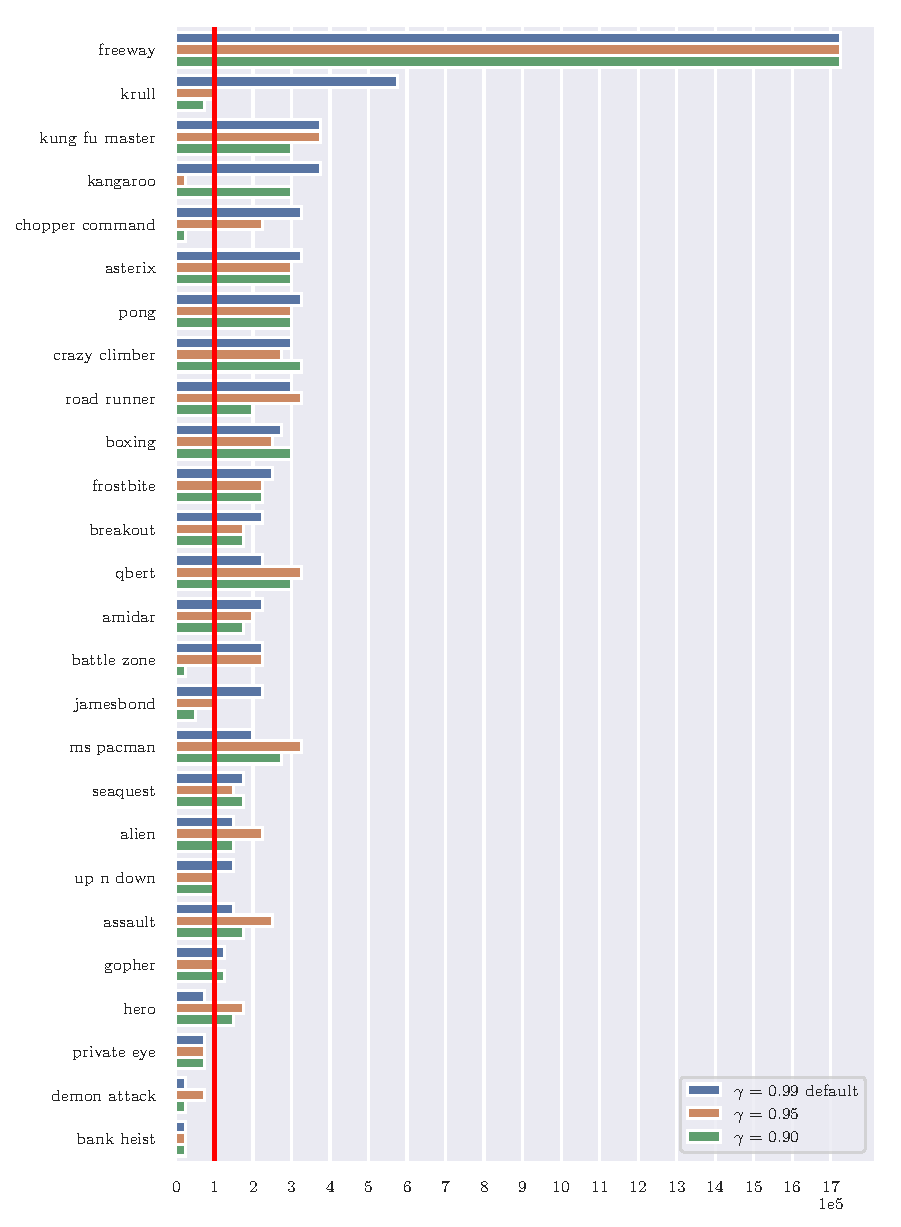
\includegraphics[width=0.9\columnwidth]{figures/graph_Effect_of_adjusting_Gamma.pdf}
\caption{Effect of adjusting $\gamma$.} 
\label{fig:adj_gamma}
\end{figure}

\begin{figure}
\centering
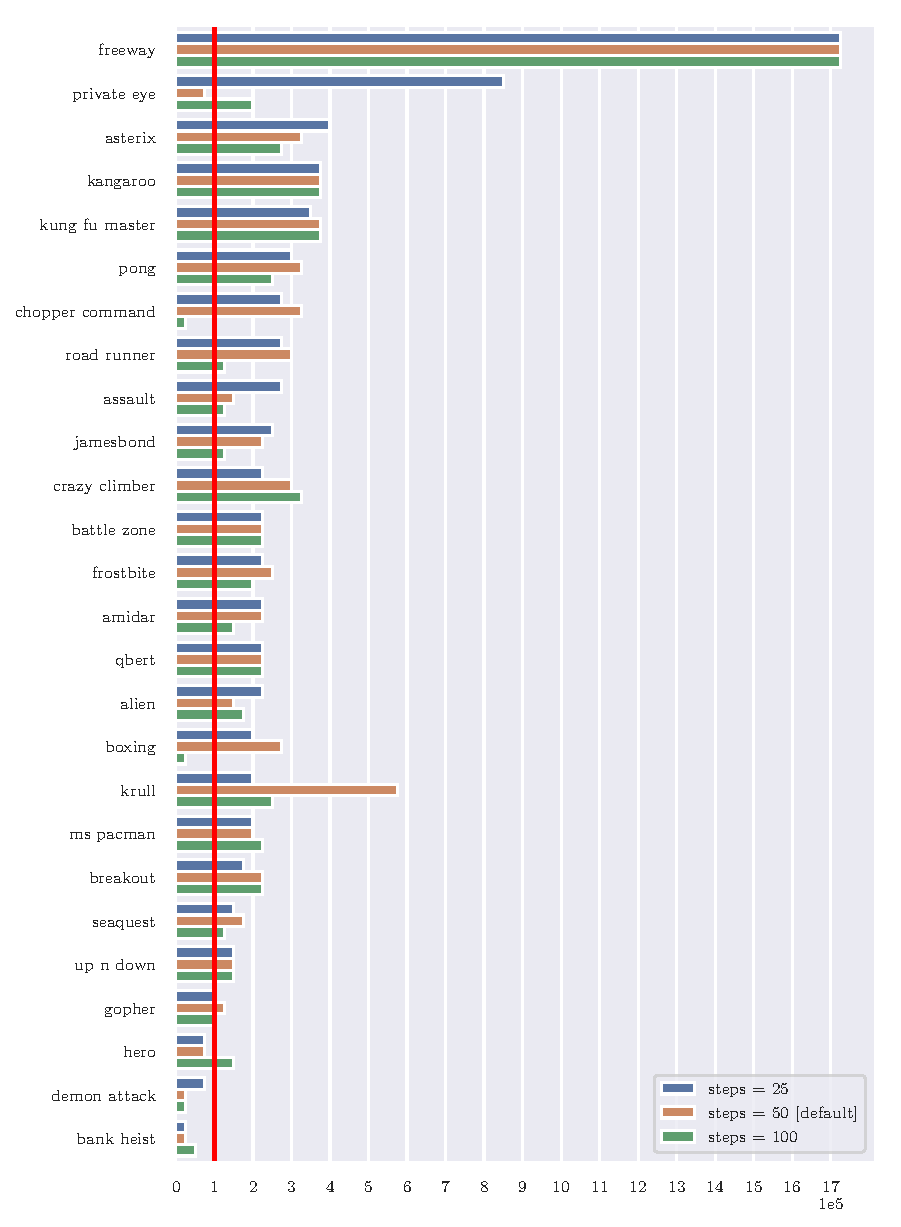
\includegraphics[width=0.9\columnwidth]{figures/graph_Effect_of_adjusting_number_of_steps.pdf}
\caption{Effect of adjusting number of steps.} 
\label{fig:adj_steps}
\end{figure}

\begin{figure}
\centering
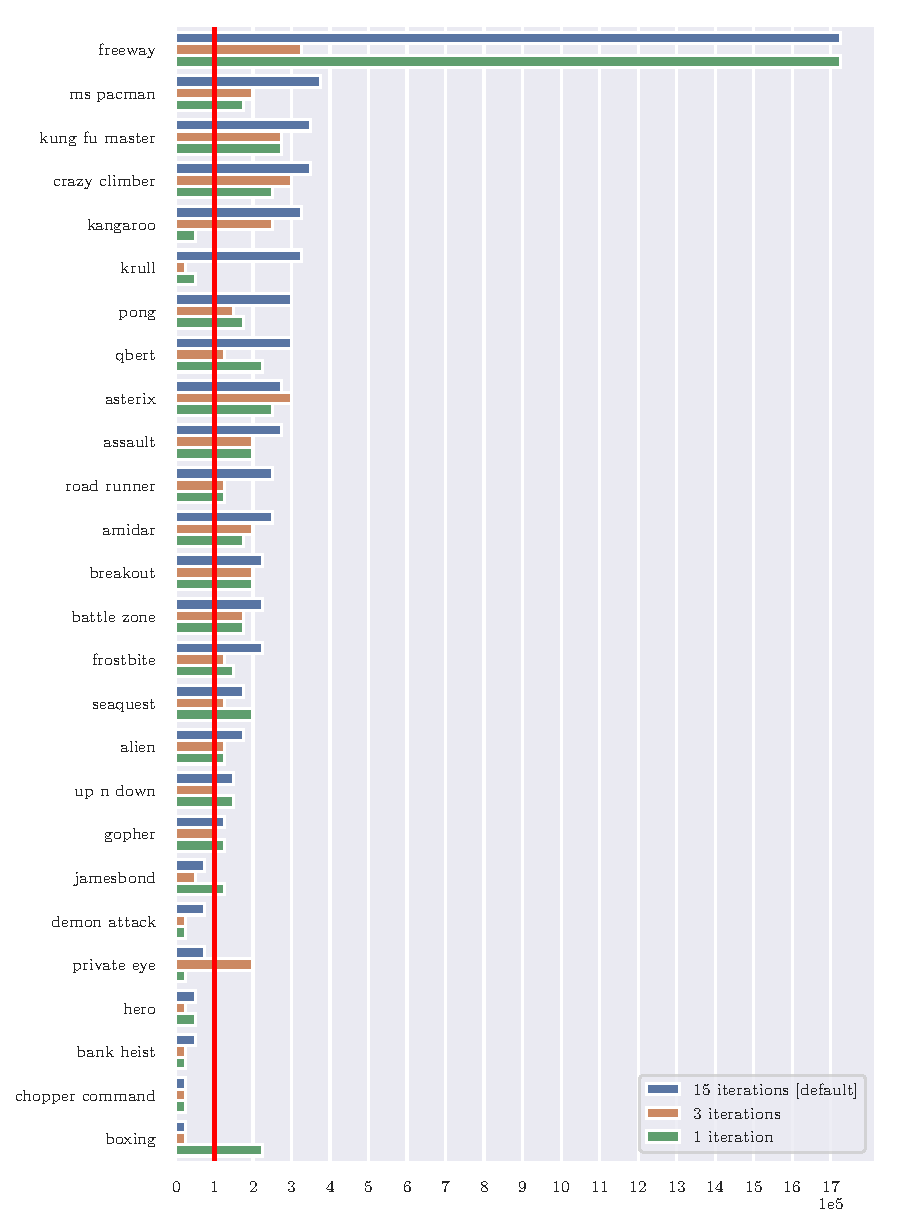
\includegraphics[width=0.9\columnwidth]{figures/graph_Effect_of_adjusting_number_of_main_loop_iterations.pdf}
\caption{Effect of adjusting number of training loops.} 
\label{fig:adj_loops}
\end{figure}


\begin{figure}
\centering
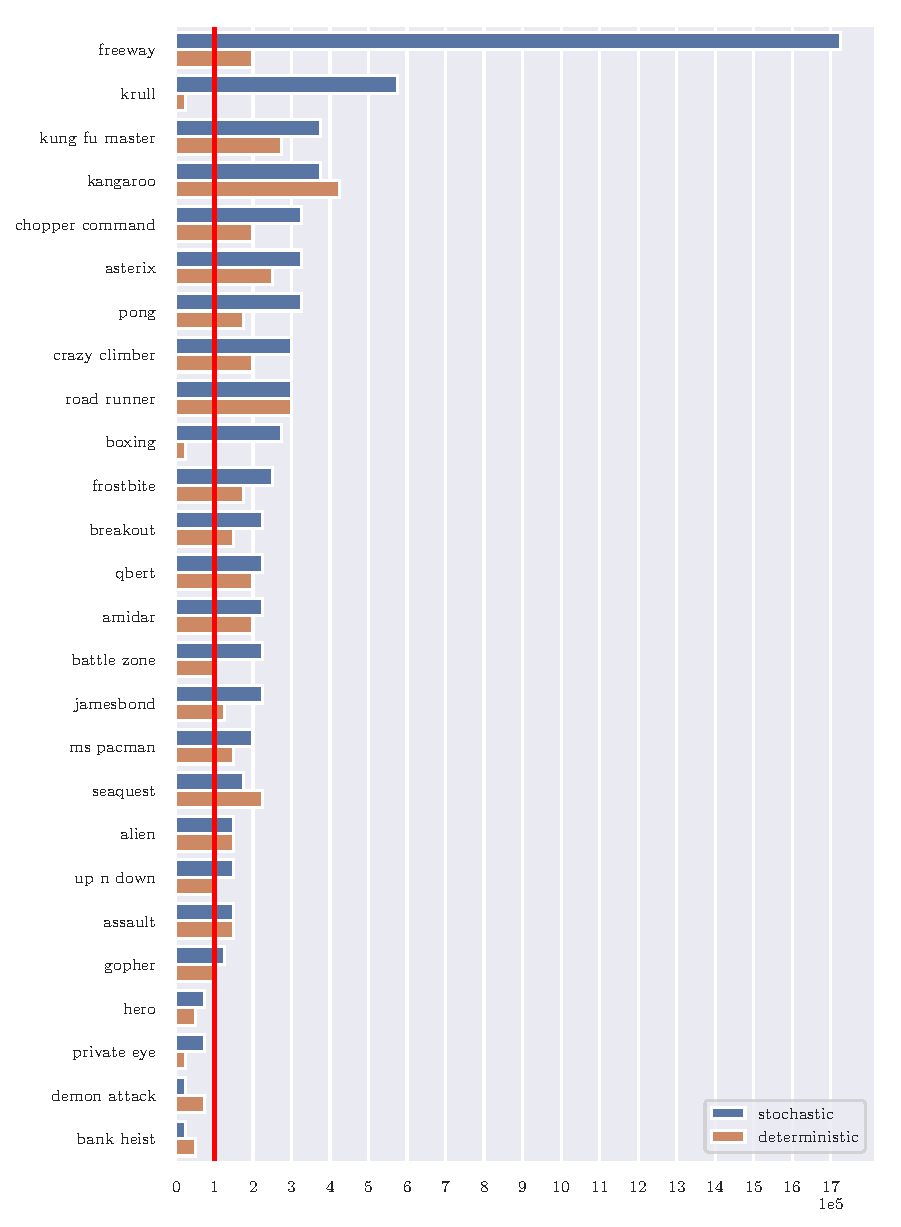
\includegraphics[width=0.9\columnwidth]{figures/graph_Effect_of_stochasticity.pdf}
\caption{Effect of stochasticity.} 
\label{fig:effects_stocha}
\end{figure}

\begin{figure}
\centering
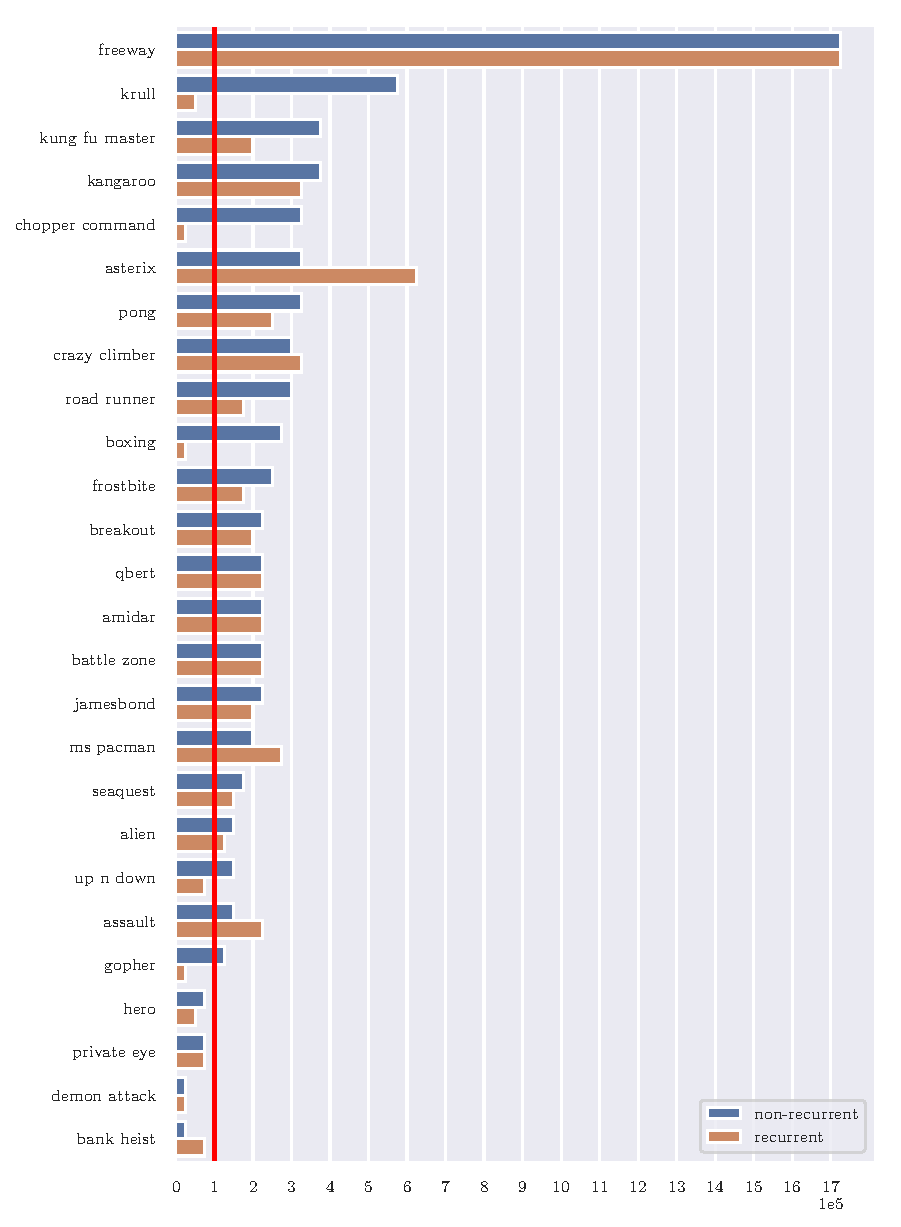
\includegraphics[width=0.9\columnwidth]{figures/graph_Effect_of_a_recurrent_architecture.pdf}
\caption{Effect of recurrence.}
\label{fig:comp_recurr}
\end{figure}

% ================= Here goes NeurIPS version ===========


\paragraph{Long model training} Our best results were obtained with much long training of models, see Figure \ref{fig:ablations2} (a) for comparison with shorter training. Due to our resources constraints other ablations were made with the short model training setting.

\paragraph{Random starts.} Using short rollouts is crucial to mitigate the compounding errors under the model. To ensure exploration SimPLe starts rollouts from randomly selected states taken from the real data buffer $\textsc{D}$. In Figure \ref{fig:Cdf} we present a comparison with an experiment without random starts and rollouts of length $1000$ on \seaquest. These data strongly indicate that ablating random starts substantially deteriorate results.  


\begin{table}
\caption{Summary of SimPLe ablations, see text for details..}
\begin{center}
  \begin{tabular}{lrr}\label{tab:ab}
model  &  best &  at least median \\
% &       &                  \\
\midrule
deterministic       &     $0$ &                $7$ \\
det. recurrent  &     $3$ &               $13$ \\
%SV2P       &     0 &                1  \\
SD         &     $8$ &               $16$ \\
SD $\gamma=0.9$     &     $1$ &               $14$ \\
default     &     $10$ &               $21$ \\
SD $100$ steps    &     $0$ &               $14$ \\
SD $25$ steps     &     $4$ &               $19$ \\
\bottomrule
\end{tabular} 
\end{center}
\end{table}


\newcommand{\mywidth}{3.0in}

\begin{figure}
\begin{tabular}{cc}
\subfloat[Effect of extended model training.]{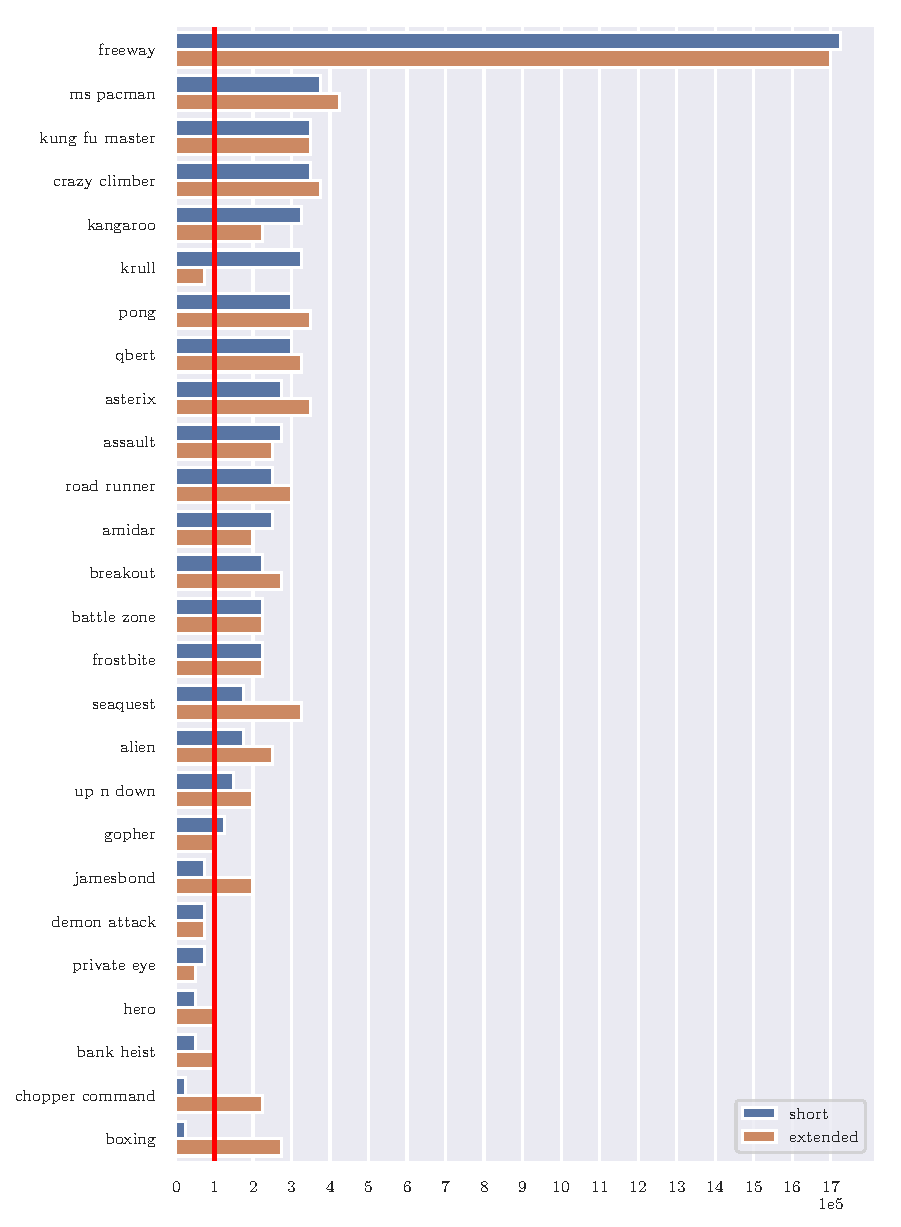
\includegraphics[width = \mywidth]{figures/graph_Effect_of_extended_model_training.pdf}} &


\subfloat[Remove]{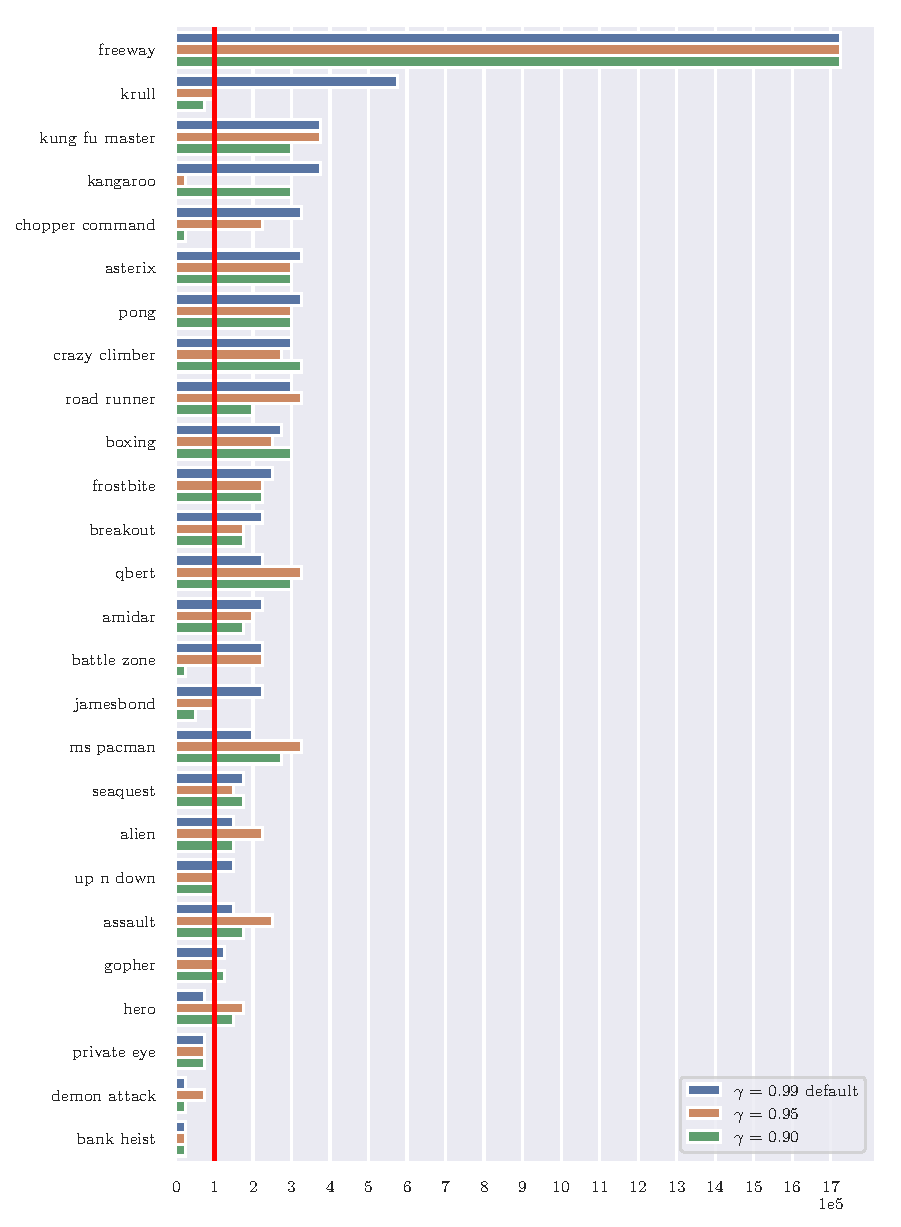
\includegraphics[width = \mywidth]{figures/graph_Effect_of_adjusting_Gamma.pdf}}

\end{tabular}
\caption{Ablations part 2 \label{fig:ablations2}}
\end{figure}
% =================================



\subsection{Number of Frames / Rainbow}\label{qualitative_analysis}

What graph here?





\subsection{Qualitative Analysis}\label{qualitative_analysis}
This section provides a qualitative analysis and case studies of individual games. We emphasize that we did not adjust the method nor hyperparameters individually for each game, but we provide specific qualitative analysis to better understand the predictions from the model.\footnote{We strongly encourage the reader to watch accompanying videos \url{https://goo.gl/itykP8}} 

\begin{figure}[t]
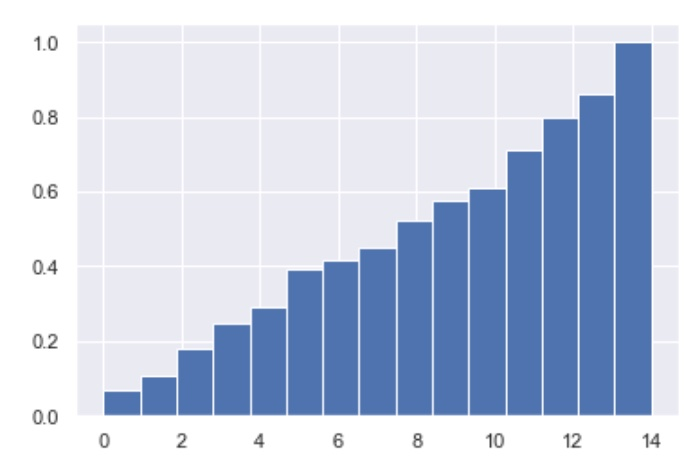
\includegraphics[width=0.90\columnwidth]{figures/cdf_max_attained}\hfill
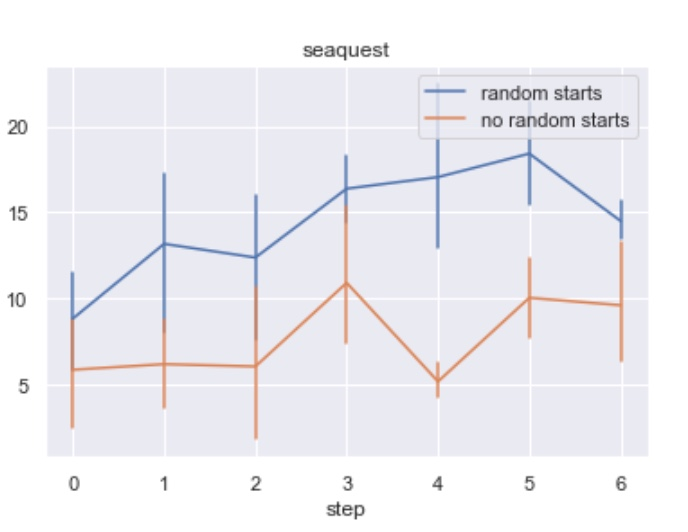
\includegraphics[width=0.90\columnwidth]{figures/random_starts_ablations}
\caption{(up) CDF of the number of iterations to acquire maximum score. The vertical axis represents the fraction of all games. (down) Comparison of random starts vs no random starts on \seaquest\, (for better readability we clip game rewards to $\{-1,0,1\}$). The vertical axis shows a mean reward and the horizontal axis the number of iterations of Algorithm \ref{alg:basic_loop}. }
\label{fig:Cdf}
\end{figure}

\paragraph{Solved games.} 
The primary goal of our paper was to use model-based methods to achieve good performance within a modest budget of $100$k interactions. For two games, \pong\, and \freeway, our method, SimPLe, was able to achieve the maximum score.

\paragraph{Exploration.}  \freeway\, is a particularly interesting game. Though simple, it presents a substantial exploration challenge. The chicken, controlled by the agents, is quite slow to ascend when exploring randomly as it constantly gets bumped down by the cars (see the left video \url{https://goo.gl/YHbKZ6}). This makes it very unlikely to fully cross the road and obtain a non-zero reward. Nevertheless, SimPLe is able to capture such rare events, internalize them into the predictive model and then successfully learn a successful policy.

However, this good performance did not happen on every run. We conjecture the following scenario in failing cases. If at early stages the entropy of the policy decayed too rapidly the collected experience stayed limited leading to a poor world model, which was not powerful enough to support exploration (e.g. the chicken disappears when moving to high). In one of our experiments, we observed that the final policy was that the chicken moved up only to the second lane and stayed waiting to be hit by the car and so on so forth. 

\paragraph{Pixel-perfect games.} In some cases (for \pong, \freeway, \breakout) our models were able to predict the future perfectly, down to every pixel. This property holds for rather short time intervals, we observed episodes lasting up to 50 time-steps. Extending it to long sequences would be a very exciting research direction. See videos \url{https://goo.gl/uyfNnW}.

\paragraph{Benign errors.} Despite the aforementioned positive examples, accurate models are difficult to acquire for some games, especially at early stages of learning. However, model-based RL should be tolerant to modest model errors. Interestingly, in some cases our models differed from the original games in a way that was harmless or only mildly harmful for policy training.

For example, in \bowling\, and \pong, the ball sometimes splits into two. While nonphysical, seemingly these errors did not distort much the objective of the game, see Figure \ref{fig:pong} and also \url{https://goo.gl/JPi7rB}.

\begin{figure}[htbp]
\makebox[\columnwidth]{%
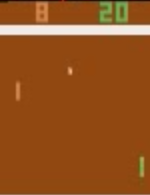
\includegraphics[width=0.25\columnwidth]{figures/pong_ball_frame1.png}%
\hfill    
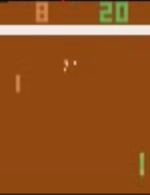
\includegraphics[width=0.25\columnwidth]{figures/pong_ball_frame2.png}%
\hfill    
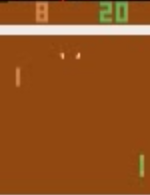
\includegraphics[width=0.25\columnwidth]{figures/pong_ball_frame3.png}%
\hfill    
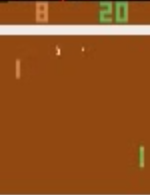
\includegraphics[width=0.25\columnwidth]{figures/pong_ball_frame4.png}%
}%
\hfill  

\caption{Frames from the \pong\ environment. }
\label{fig:pong}
\end{figure}


In \kungfumaster\, our model's predictions deviate from the real game by spawning a different number of opponents, see Figure \ref{fig:boxing}. In \crazyclimber\, we observed the bird appearing earlier in the game. These cases are probably to be attributed to the stochasticity in the model. Though not aligned with the true environment, the predicted behaviors are plausible, and the resulting policy can still play the original game.

\begin{figure}[htbp]
\makebox[\columnwidth]{%
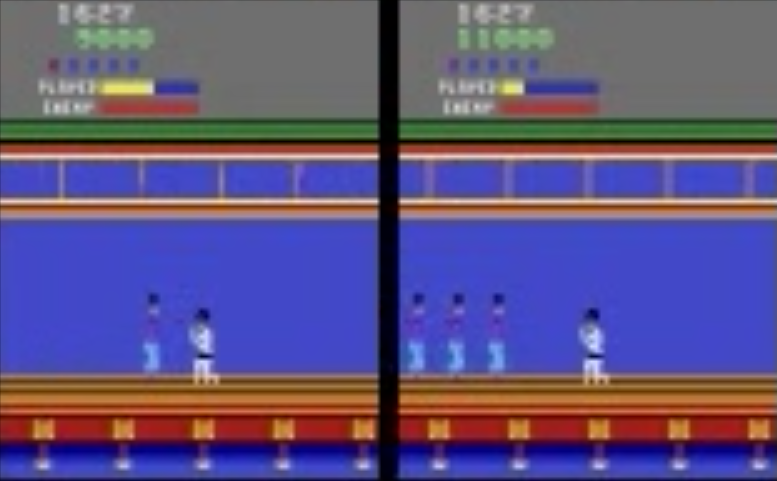
\includegraphics[width=0.50\columnwidth]{figures/kungfu1.png}%
\hfill    
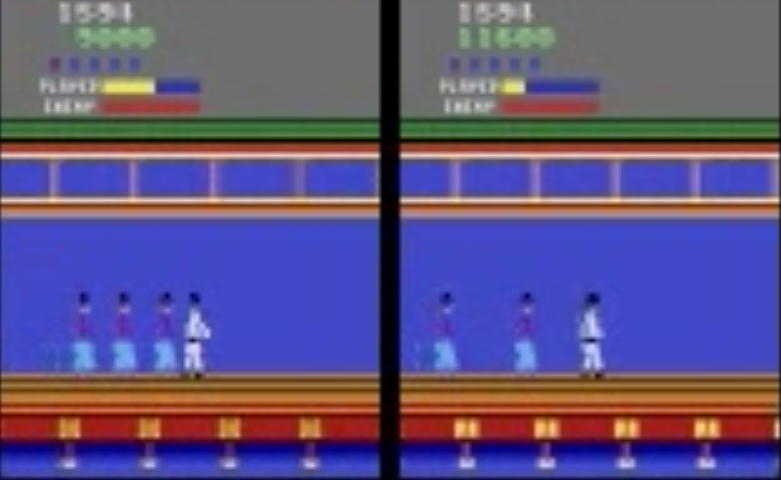
\includegraphics[width=0.50\columnwidth]{figures/kungfu2.png}%
}%
\caption{Frames from the \kungfumaster\ environment (left) and its model (right). }
\label{fig:boxing}
\end{figure}

\paragraph{Failures on hard games.}
On some of the games, our models simply failed to produce useful predictions. We believe that listing such errors may be helpful in designing better training protocols and building better models. The most common failure was due to the presence of very small but highly relevant objects. For example, in \atlantis\, and \battlezone\, bullets are so small that they tend to disappear. Interestingly, \battlezone\, has pseudo-3D graphics, which may have added to the difficulty. See videos \url{https://goo.gl/uiccKU}.

Another interesting example comes from \privateeye\, in which the agent traverses different scenes, teleporting from one to the other. We found that our model generally struggled to capture such large global changes.